In order to generate a system that could be used in diverse platforms, an abstraction level in which all of them could fall is required. Simple and compound actions are used to achieve this goal. Simple actions are actions that are considered as primitives: they are used as building blocks. As a consequence, these actions are described in the system and are the ones whose parameters are changed to embed the emotions. Their description specifies mandatory and optional parameters that are required to execute an action. These parameters are modified accordingly to the information provided by the emotional parameters. Compound actions are actions that are created from simple actions and other compound actions. For example, two actions that are executed in parallel are considered as compound actions. These actions are not always implemented in the system. They can be described in the action messages without being implemented. If a compound action is used often, it could be implemented in the system. The implementation describes action's parameters, other compound actions, simple actions, and mapping between actions and parameters.

A set of simple actions to be implemented were selected to test the system, considering the capabilities of Keepon and Triskarino. The eight actions selected were: \textit{move body}, \textit{oscillate body}, \textit{move shoulder}, \textit{oscillate shoulder}, \textit{move torso}, \textit{oscillate torso}, and \textit{do nothing}. Description for each action, its mandatory parameters and optional parameters are presented in Table~\ref{table:actions_implemented}.

\begin{table}
\centering
\caption{Description of the seven simple actions implemented, and their respective parameters, where P is 2D position, V is 2D velocity vector and angular velocity, and T is time}
\label{table:actions_implemented}
\begin{tabular}{|c|p{3.9cm}|p{1.4cm}|}
\hline
\textbf{Action Name}& \textbf{Description} &\textbf{Parameter(s)} \\
\hline
Do nothing & It waits for a time $t$ before it is terminated. It could be seen as a delay.  & $T$\\
\hline
Move body & It moves the platform from its current position $a$ to a desired position $b$. & $P$, and $V$\\
\hline
Oscillate body & It generates an oscillation in the whole platform by an angle $\theta$. &  $\theta$ and $V$ \\
\hline
Move shoulder & It moves the shoulders to a desired angle $\theta$. It is considered as angular movement. & $\theta$ and $V$ \\
\hline
Oscillate shoulder & It oscillates the shoulders by a given angle $\theta$ & $\theta$ and $V$\\
\hline
Move torso & It moves the torso to a desired angle in $yaw$, $pitch$ and $roll$& $yaw$, $pithc$, $roll$ and $V$\\
\hline
Oscillate torso & It oscillates the shoulders by a given angle $\theta$ & $\theta$ and $V$\\  
\hline
\end{tabular}
\end{table}

To exemplify the use of these actions, let us consider a sequence of movements illustrated in Figure~\ref{fig:triskar_test}. This sequence of movements corresponds to an adaptation of the first part of the balcony scene of Shakespeare's Romeo and Juliet play~\cite{RAndJ}. The fist part of this scene is characterized by strong changes in Romeo's emotional state, thus it was selected as a significant test for the system.  
\begin{figure}
	\centering
	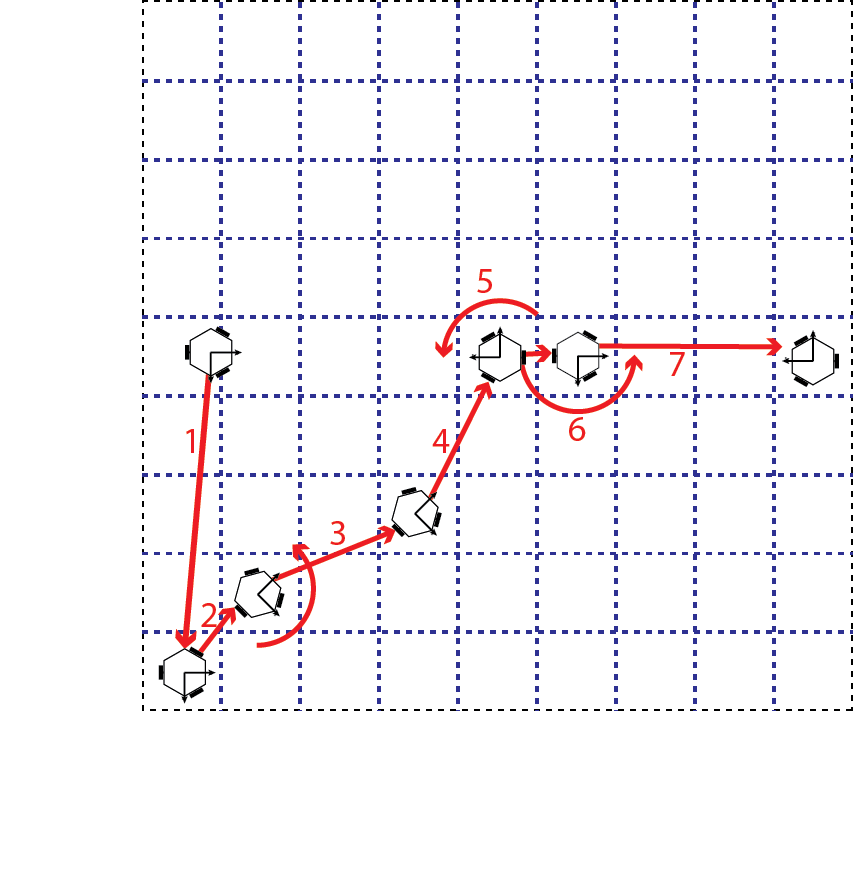
\includegraphics[width=0.45\textwidth]{./Images/FourthCaseSceneB.png}
	\caption{Sketch of Romeo's movements for the balcony scene in Romeo and Juliet play. The arrows show the direction of the movements, and the numbers their position in the sequence.}
	\label{fig:triskar_test}
\end{figure} 
However, just body movements would not exploit the other movements of the platform neither test the whole system. Thus, additional movements are added to illustrate and test the system. A partial view of the whole sequence of actions is illustrated in Figure~\ref{fig:sequence_actions}. The first node corresponds to the first action in Figure~\ref{fig:triskar_test}. The second node corresponds to a compound action created by the parallel execution of the simple action \textit{move body} and other compound actions.

\begin{figure}
	\centering
	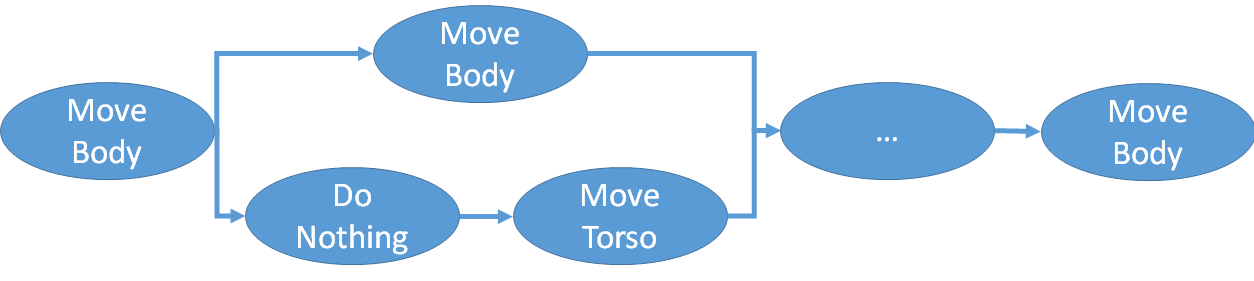
\includegraphics[width=0.5\textwidth]{./Images/sequenceActions.png}
	\caption{Sequence of simple actions for the movements depicted in Figure~\ref{fig:triskar_test}.}
	\label{fig:sequence_actions}
\end{figure}
